\begin{figure}
    \begin{center}
    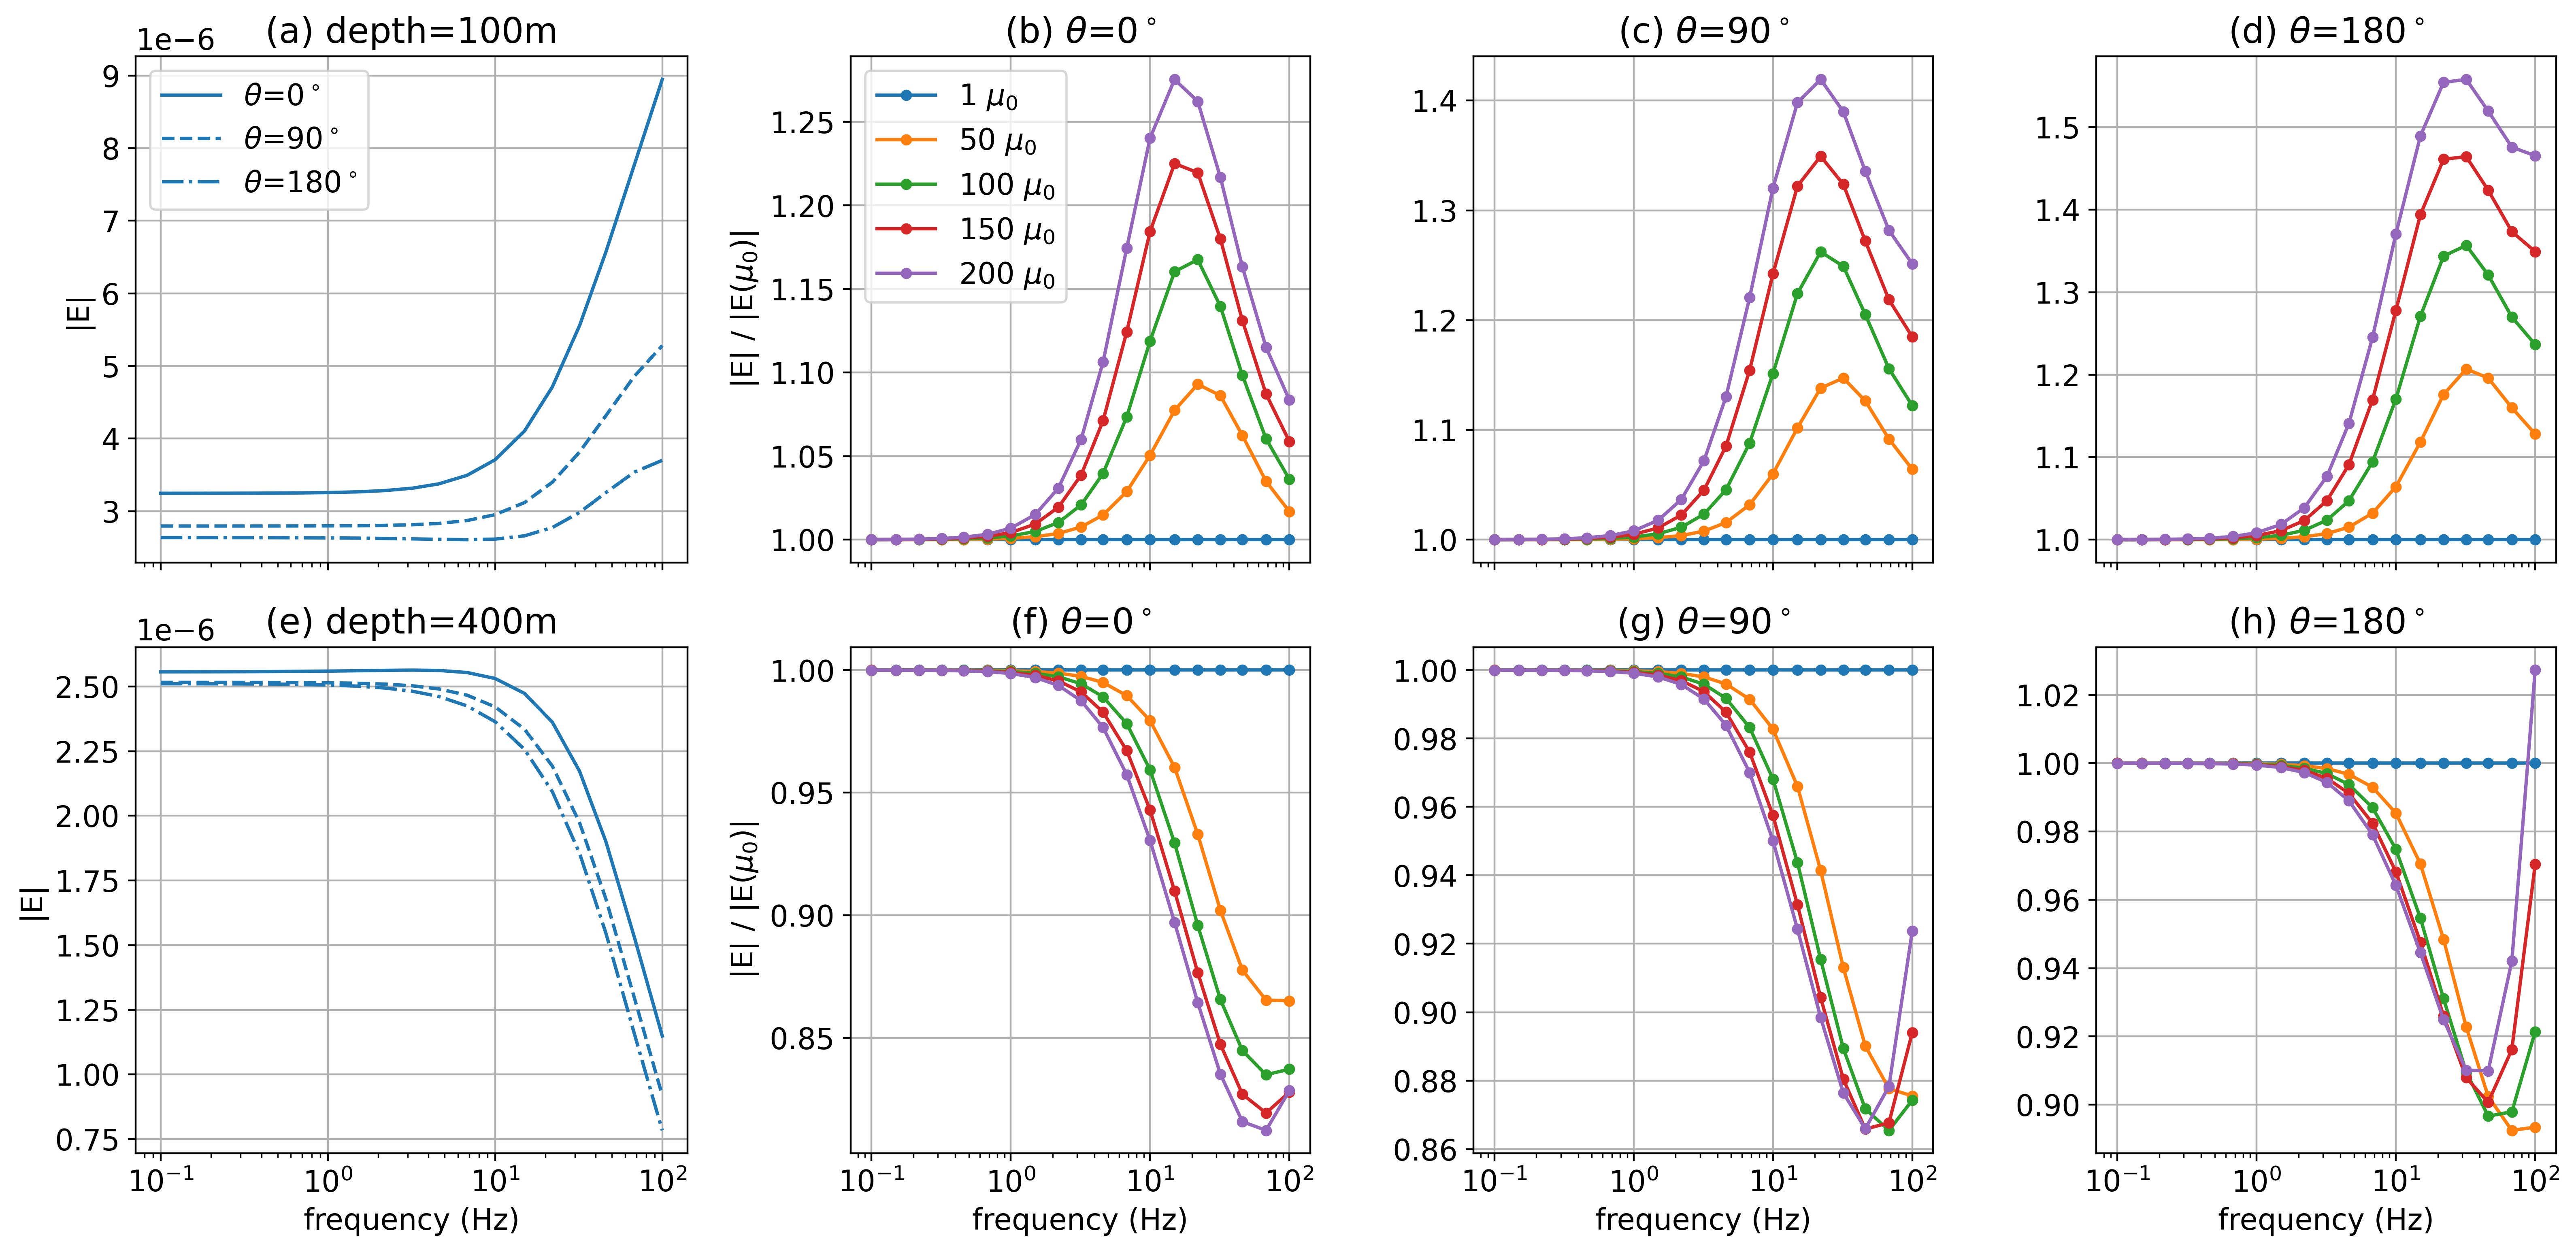
\includegraphics[width=\textwidth]{figures/excitation-freq.png}
    \end{center}
\caption{
    Amplitude of the average electric field over a test volume that is the same as was used in Figure \ref{fig:excitation-time-integrated}. The different line-styles in (a) and (e) indicate different azimuths for the non-permeable well ($\mu_0$). Panels (b), (c), and (d) show the ratio of the amplitude of the electric field with respect to the non-permeable well ($\mu=\mu_0$) for the test volume centered at a depth of 100m. Panels (f), (g) and (h) show the ratios of the electric field amplitude for the test volume centered at 400m depth.
}
\label{fig:excitation-freq}
\end{figure}



